\begin{frame}{Reservoir Computing}
	\par In 2001, two works were proposed independently and at different times and countries. However, both dealt with the concept of Reservoir Computing, with slightly different models. Echo State Networks were presented in a more general way, in a mathematical and engineering approach, demonstrating the use of Reservoir Computing for time series prediction tasks. While in the same year the Liquid State Machine model was proposed by Wolfgang Maass, Thomas Natschläger and Henry Markram, reaching a result very similar to the ESN.
\end{frame}

\begin{frame}{Liquid State Machine}	
	\par  \textit{"Liquid State Machines can be a type of Reservoir Computing(RC) model, similar to Echo State Networks(ESNs), they can leverage the dynamics of a recurrent neural network with randomly connected neurons to process sequential and time-series data efficiently. LSMs were introduced as an extension of ESNs, incorporating additional principles inspired by biological neural networks."} \cite{3}
\end{frame}

\begin{frame}{Echo State Networks}
	\par Echo State Networks were proposed by Herbert Jaeger in his work "The 'echo state' approach to analyzing and training recurrent neural networks". 
	In this work, he demonstrates a dynamics reservoir architecture with just 3 layers:
	\begin{itemize}
		\item Input Layer
		\item Reservoir Layer
		\item Output Layer
	\end{itemize}
\end{frame}

\begin{frame}{Objectives}
	\par The objective of an Echo State Network is to maximize $W_{out}$ based on the dynamics generated by the reservoir, recovering data from previous stages and allowing the identification of patterns based on the given history.
\end{frame}

\begin{frame}{General Process Diagram}
	\begin{figure}
		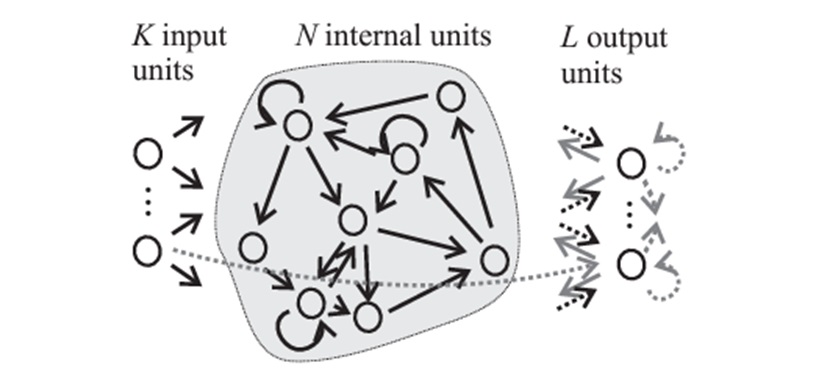
\includegraphics[width=0.9\textwidth, height=0.7\textheight]{images/diagramaESN.jpg}
		\caption{The Jaeger model - Source:\cite{1}}
	\end{figure}
\end{frame}


\begin{frame}{Architecture}
	\begin{figure}
		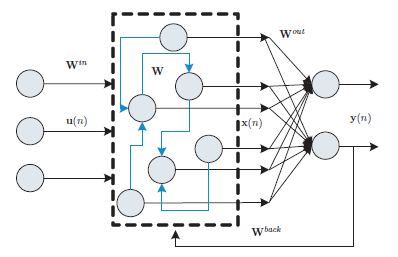
\includegraphics[width=.6\textwidth]{images/arquitetura_.png}
		\caption{Source: \cite{4}}
	\end{figure}
\end{frame}

\begin{frame}
	\frametitle{Algorithm}
	
	\only<1>{
		\par According to \cite{4} Consider a discrete-time recurrent neural network with K input units, N internal units and L outputs, as depicted in Figure 1.
		The vector $u(n) =  [u_{\text{1}}(n)...u_{\text{K}}(n)]^T$ denotes the activations of the input units, which are transmitted to the internal neurons by means of a linear combination. The weight matrix $W^{in} \in R^{N x K}$ specifies the coefficients of such combinations.
	}
	\only<2>{
		\par The internal layer, also called dynamical reservoir, is composed of fully-connected nonlinear units whose activations, given by x(n) = $[x_1(n)...x_N(n)]^T$ , correspond to the network states, and are updated as follows:
		$x(n + 1) = f(\textbf{W}^{in}\textbf{u}(n + 1) + \textbf{Wx}(n) + \textbf{W}^{back}\textbf{y}(n))$ ,
	}
	\only<3>{
		\par where $\textbf{W} \in R^{N x N}$ brings the weights of the connections within the reservoir, $\textbf{W}^{back} \in R^{N x L}$ contains the weights associated with the connections that project the output samples back to the internal units, and $\textbf{f}(\cdot) = (\textit{f }_{1}(\cdot), ..., \textit{f}_N(\cdot))$ denotes the activation functions of the internal units.
	}
	\only<3>{
		\par Finally, the outputs of the network, represented by the vector$y(n) = [y_1(n) ... y_L(n)]^T$, are determined by the following expression:
		$y(n + 1) = f^{out}(\textbf{W})^out \textbf{x}(n + 1)$, where $\textbf{W}^{out} \in R^{L x N}$ is the output weight matrix and 		
		$\textbf{f}(\cdot) = (\textit{f }_{1}^{out}(\cdot), \dots´, \textit{f }_{L}^{ out}(\cdot))$ especifies the activation functions of the output units.
	}
\end{frame}

\begin{frame}{Echo State}
	\par According to \cite{4} Jaeger demonstrated two sufficient conditions regarding echo states:
	
	\begin{itemize}
		\item \textbf{The first condition} determines that for an RNN to present the echo state property, the largest singular value of the internal weight matrix W must be less than unity.
		\item \textbf{The second condition} establishes the non-existence of echo states in terms of the spectral radius (the largest among the absolute eigenvalues) of the internal weight matrix W: if $||W||| > 1$, then the network has no echo states
	\end{itemize}
	
\end{frame}

\begin{frame}{Applications}
	\par ESNs have gained notoriety and have been used to solve the most diverse problems. But the main focus of use is on:
	\begin{itemize}
		\item Time series forecasting.
		\item Signal processing.
		\item Pattern Recognition.
		\item Natural Language Processing (NLP).
	\end{itemize}
\end{frame}

\begin{frame}{Practical presentation}
	\par The model used for testing is accessible on the website \url{https://mantas.info/code/simple_esn/} \cite{2} from which it was originally derived. This model is designed to generate a neural network that, when provided with an audio file containing a melodic sequence as input, produces an output that closely resembles the original audio in its predictions. The resulting prediction is saved in a new file for comparison.
\end{frame}

\begin{frame}{Conclusions}\label{sec:conclusoes}
	Based on the research carried out, it was demonstrated in the works read that Echo State Networks enable substantial gains when applied to prediction tasks involving historical data, such as time series prediction and Natural Language Processing. They are capable of recovering short-term memory states and reducing the possibility of overfitting and gradient explosion.
\end{frame}
